\chapter{Apprendimento democratizzato: concetti}\label{ch:chapter2}
L'algoritmo proposto utilizza lo schema bottom-up per eseguire in modo iterativo l'apprendimento locale risolvendo problemi di apprendimento personalizzati e aggiornando gerarchicamente i modelli generalizzati per gruppi a livelli superiori.\\
Diversamente dall'algoritmo di apprendimento federato, il Dem-AI introduce una struttura gerarchica auto-organizzante per risolvere compiti di apprendimento complessi singoli/multipli mediando i contributi di un gran numero di agenti di apprendimento in un apprendimento collaborativo. Secondo le differenze nelle loro caratteristiche, gli agenti di apprendimento formano gruppi appropriati che possono essere specializzati affinché agenti simili affrontino i compiti di apprendimento. Questi gruppi specializzati sono auto-organizzati in una struttura gerarchica e costruiscono collettivamente la conoscenza di apprendimento generalizzata condivisa per migliorare le loro prestazioni di apprendimento riducendo i problemi individuali dovuti ai dati locali sbilanciati e altamente personalizzati. In particolare, il sistema di apprendimento consente ai nuovi membri del gruppo di accelerare il loro processo di apprendimento con la conoscenza del gruppo esistente e incorporare le loro nuove conoscenze di apprendimento espandendo la capacità di generalizzazione dell'intero gruppo. In questi sistemi ogni agente è libero di unirsi ad uno dei qualsiasi gruppi e possiedono lo stesso potere inteso come numero dei componenti che varierà poi nel tempo.\\
Consideriamo quindi i punti principali del Dem-AI.\\\\
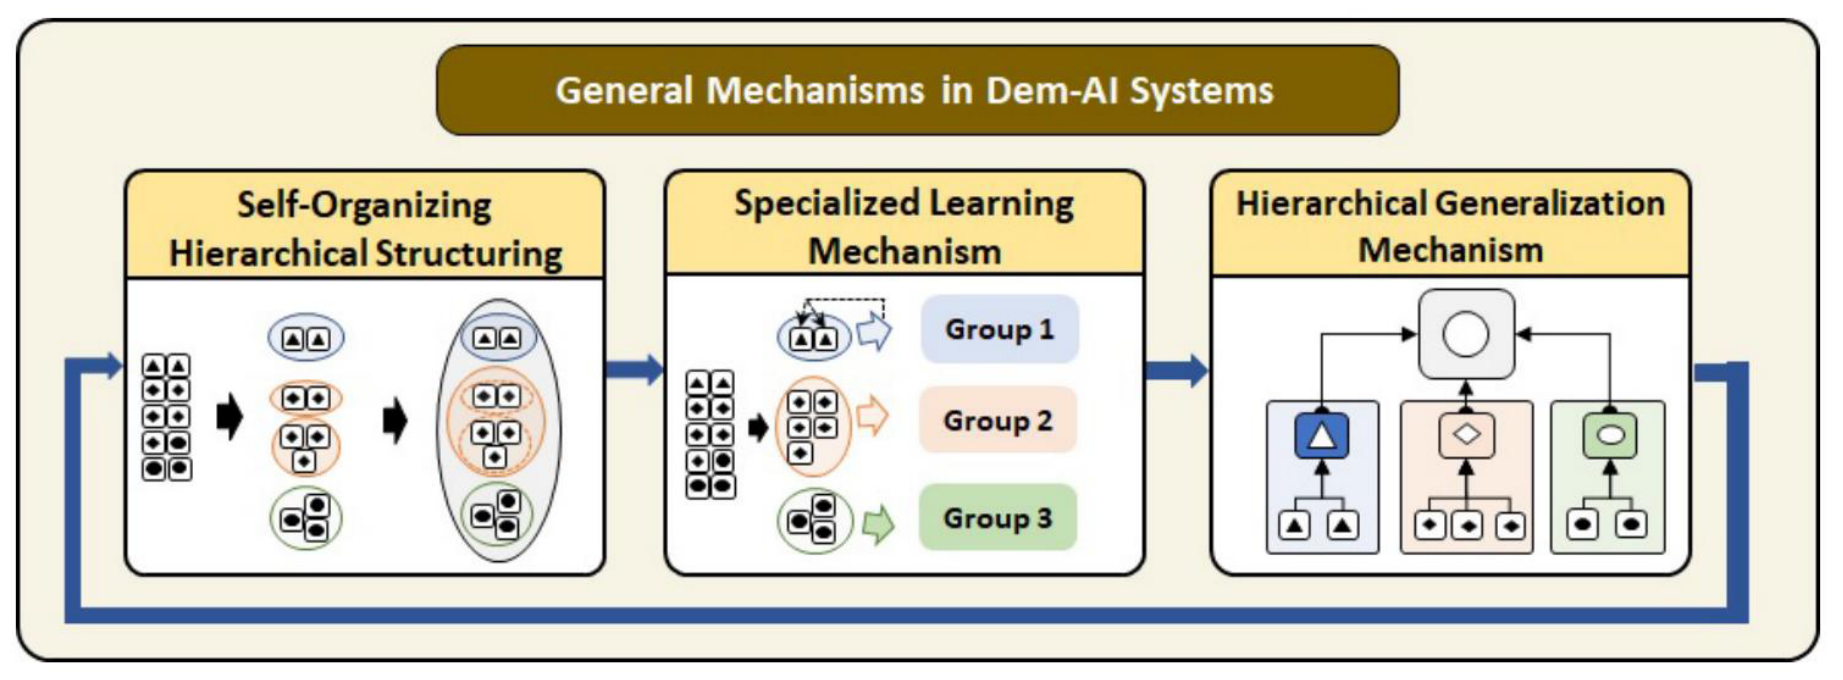
\includegraphics[scale=0.25]{DemIA}
\captionof{figure}{Meccanismi generali del sistema DemIA} \vspace{0.5cm}


\begin{itemize}

  \item Definizione ed obiettivo\\
  L'apprendimento democratizzato studia processi duali ,accoppiati e operanti insieme, specializzato-generalizzato in una struttura gerarchica auto-organizzante di sistemi di apprendimento distribuiti su larga scala. I processi specializzati e generalizzati devono operare congiuntamente verso un obiettivo di apprendimento finale identificato come l'esecuzione di un apprendimento collettivo da agenti di apprendimento prevenuti, che si impegnano ad apprendere dai propri dati utilizzando le loro limitate capacità di apprendimento. In quanto tale, l'obiettivo finale di apprendimento del sistema Dem-AI è stabilire un meccanismo per risolvere collettivamente compiti di apprendimento complessi comuni (singoli o multipli) da un gran numero di agenti di apprendimento
  \item Processo specializzato\\
  Questo processo viene utilizzato per sfruttare le capacità di apprendimento specializzate degli agenti di apprendimento e dei gruppi specializzati sfruttando i dati raccolti. Incorporando la conoscenza generalizzata dei gruppi di livello superiore creati dal meccanismo di generalizzazione, gli agenti di apprendimento possono aggiornare i parametri del loro modello per ridurre il bias nel loro apprendimento personalizzato.
Pertanto, l'obiettivo di apprendimento personalizzato ha come obiettivi: eseguire un apprendimento specializzato e riutilizzare la conoscenza gerarchica generalizzata disponibile.
  \item Processo generalizzato\\
  Il meccanismo di generalizzazione incoraggia i membri del gruppo a condividere la conoscenza quando svolgono compiti di apprendimento con caratteristiche simili e costruiscono livelli gerarchici di conoscenza generalizzata. La conoscenza gerarchica generalizzata aiuta il sistema Dem-AI a mantenere la capacità di generalizzazione per ridurre il bias degli agenti di apprendimento e affrontare in modo efficiente i cambiamenti ambientali o eseguire nuovi compiti di apprendimento.
  
  \item Struttura gerarchica auto-organizzante\\
  La struttura gerarchica dei gruppi specializzati e le relative conoscenze generalizzate sono costruite e regolate secondo un principio di autoorganizzazione basato sulla somiglianza degli agenti di apprendimento. In particolare, questo principio governa l'unione di piccoli gruppi per formare un gruppo più grande che alla fine migliora le capacità di generalizzazione di tutti i membri. Pertanto, i gruppi specializzati ai livelli più alti nella struttura gerarchica hanno più membri e possono costruire una conoscenza più generalizzata e meno distorta adattandosi più rapidamente ai nuovi ambienti.
  
\item Transizione nel duplice processo specializzato-generalizzato\\
Il processo specializzato diventa sempre più importante rispetto al processo generalizzato durante il periodo di formazione. Di conseguenza, il sistema di apprendimento non solo si evolve per acquisire capacità di specializzazione dai compiti appresi, ma perde anche la capacità di affrontare i cambiamenti ambientali come nuovi agenti di apprendimento e nuovi compiti di apprendimento. Nel frattempo, la struttura gerarchica del sistema Dem-AI è auto-organizzata e si è evoluta da un alto livello di plasticità a un alto livello di stabilità, cioè da gruppi specializzati instabili a gruppi specializzati ben organizzati. La transizione del sistema di apprendimento Dem-AI è illustrata in figura con tre sub-meccanismi iterativi come la generalizzazione, l'apprendimento specializzato e il meccanismo di strutturazione gerarchica. Di conseguenza, la transizione del processo duale specializzato-generalizzato rappresenta le fasi di un tipico quadro di apprendimento democratizzato. In quella transizione, gli agenti di apprendimento sono raggruppati in base alle somiglianze dei loro compiti di apprendimento nella fase iniziale. Quindi, il processo generalizzato aiuta nella costruzione di una conoscenza gerarchica generalizzata per i gruppi specializzati dal basso verso l'alto e incoraggia i membri del gruppo a essere vicini. Nel frattempo, i processi di apprendimento specializzati sfruttano l'apprendimento personalizzato per sfruttare i loro set di dati distorti incorporando la conoscenza di gruppo generalizzata di livello superiore dai gruppi di livello superiore a quelli di livello inferiore.

\end{itemize}
